\documentclass[11pt]{article}
\usepackage[margin=1in]{geometry}
\usepackage{amsmath,amssymb,amsthm}
\usepackage{graphicx}
\usepackage{enumitem}
\usepackage{booktabs}
\usepackage[hidelinks]{hyperref}
\usepackage{caption}
\captionsetup{font=small,labelfont=bf}

\newtheorem{theorem}{Theorem}
\newtheorem{lemma}{Lemma}
\newtheorem{proposition}{Proposition}
\newtheorem{corollary}{Corollary}
\theoremstyle{definition}
\newtheorem{definition}{Definition}
\newtheorem{remark}{Remark}

\newcommand{\Z}{\mathcal{Z}}
\newcommand{\F}{\mathcal{F}}
\newcommand{\X}[1]{X_{#1}}

\title{\vspace{-1.2em}Locality of $\mathrm{Tr}(\phi^3)$ tree amplitudes from cyclic hidden zeros\\[2pt]
\large Part III: classification of Step--$2$ $k$--zero relations}
\date{}
\author{}

\begin{document}
\maketitle
\vspace{-3.2em}

\begin{abstract}
\noindent Part~II classified the asymptotic limits on a $k$--zero $\Z^{(k)}$ by a rate vector and
showed which coefficients $a_M$ are forced to vanish on each. The vanishing of $B_n$ on
$\Z^{(k)}$ carries strictly more information than that: it descends to vanishing on each homogeneous
piece (boundary--propagator order), then on each \emph{D--subset} (born--free monomial), and within
each D--subset the $X\!\to\!0$ cuts read off explicit linear relations among the surviving
coefficients $a_M$. We classify these \emph{Step--$2$ $k$--zero relations} for $k=1,2,3$ and at the
first three boundary--propagator orders. The universal $m$--th order ``binomial trace''
\begin{equation*}
  \sum_{j=0}^{m}(-1)^{j}\;a_{\,s^{\,m-j}\,b^{\,j}}\;=\;0,
\end{equation*}
($s$ the special chord, $b$ the bare) holds at every $k$ and every $m$, and a family of per--column
and per--offset relations supplements it. For $k\ge2$ these include genuinely new relations not
visible to any cyclic rotation of the $1$--zero, e.g.\ $a_{14,14}+a_{3n,3n}-a_{14,3n}=0$ and the
cubic $a_{14,14,14}-a_{14,14,3n}+a_{14,3n,3n}-a_{3n,3n,3n}=0$ for the $2$--zero. The collected
system is the substrate on which the all--$n$ argument is to close.
\end{abstract}

\section{Setting}
We adopt the conventions of Parts~I--II. The $k$--zero based at $\{1,\dots,k{+}1\}$ has special
$s=\X{1,k+2}$, bare $b=\X{k+1,n}$, and on $\Z^{(k)}$ the bridge chords are governed by
\begin{equation}\label{eq:constr}
  \X{k+1,\ell}=\X{1\ell}-s,\quad \X{k+1,n}=-s,\quad
  \X{i\ell}=\X{k+1,\ell}+\X{i,k+2},\quad \X{in}=\X{i,k+2}-s,
\end{equation}
for $i=2,\dots,k$ and $\ell=k{+}3,\dots,n{-}1$. The independent coordinates on $\Z^{(k)}$ are
$\{s\}\cup\{\X{i,k+2}\}\cup\{\X{1\ell}\}\cup\{\text{born--free}\}$ (Part~II, Eq.~(5)).

\subsection{Boundary--propagator grading}\label{sec:bp}
A \emph{boundary propagator} is any chord touched by \eqref{eq:constr}: explicitly the special, the
bare, the offsets $\X{i,k+2}$ ($i\ge2$), and the bridges $\X{1\ell},\X{i\ell},\X{k+1,\ell}$
($\ell\in\{k{+}3,\dots,n\}$). For each multiset $M$ of size $n-3$, let $|M|_{\mathrm{BP}}$ denote
the number of boundary--propagator factors in $M$ (with multiplicity). Under a uniform rescaling
$\X{ij}\mapsto\lambda\X{ij}$ of all boundary propagators, the term $a_M/\prod\X{c}$ scales as
$\lambda^{-|M|_{\mathrm{BP}}}$. Hence
\begin{equation*}
  B_n\big|_{\Z^{(k)}}\;=\;\sum_{m\ge0}B_n^{(m)},\qquad
  B_n^{(m)}=\sum_{|M|=n-3,\ |M|_{\mathrm{BP}}=m}\frac{a_M}{\prod_{c\in M}\X{c}}.
\end{equation*}
The BCFW homogeneity lemma of note~12 (the $z$--scaling argument) forces $B_n^{(m)}|_{\Z^{(k)}}=0$
for every $m$ independently. We focus on $m=1,2,3$, where the relations are most informative.

\subsection{D--subsets}
Within a fixed $B_n^{(m)}$, the born--free coordinates factor out: every term carries a unique
born--free monomial $\prod\X{c}^{-\nu_c}$ with $c$ born--free. Collecting terms by their born--free
monomial yields the D--subsets. Each D--subset is a finite sum of boundary--propagator pieces
multiplied by a common born--free factor, and \emph{each D--subset vanishes independently}: this is
the proposition of note~18 (split chord variables into boundary propagators $x$ and free $y$;
$L(x)=0$ does not depend on $y$, so the vanishing factorises per $y$--monomial).

For brevity we present the relations at the level of the boundary--propagator skeletons; each
relation should be read as holding inside every D--subset that contains the listed pattern
(i.e.\ for every choice of accompanying born--free factor).

\begin{figure}[t]
  \centering
  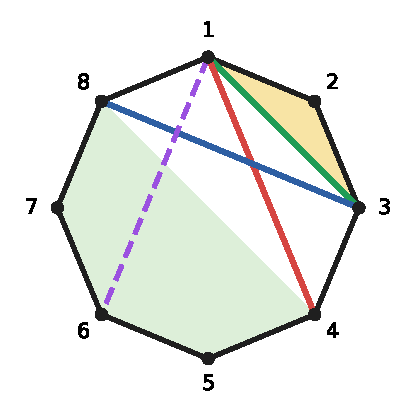
\includegraphics[width=0.34\textwidth]{figures/bp_structure.pdf}
  \caption{A $2$--zero diagram ($n=8$, $k=2$). Special $\X{1,4}$ (red), bare $\X{3,8}$ (blue),
  enclosing chord $\X{1,3}$ (green). Boundary propagators are the highlighted/dashed chords; the
  pale--green region carries the born--free factor of any D--subset.}
  \label{fig:bp}
\end{figure}

\section{The binomial--trace relation}
\begin{theorem}[Binomial trace]\label{thm:bintrace}
For every $k\ge1$, every $n>k+2$, and every $m\ge1$, the $k$--zero relations include
\begin{equation}\label{eq:bintrace}
  \sum_{j=0}^{m}(-1)^{j}\;a_{\underbrace{s,\dots,s}_{m-j},\underbrace{b,\dots,b}_{j}}\;=\;0,
\end{equation}
where $s=\X{1,k+2}$ is the special and $b=\X{k+1,n}$ is the bare.
\end{theorem}
\begin{proof}
At order $m$ the boundary--propagator subskeletons composed solely of special and bare contribute
$\sum_{j=0}^{m}a_{s^{m-j}b^j}\big/(s^{m-j}\,b^j)$. By \eqref{eq:constr}, $b=-s$, so
$1/(s^{m-j}b^j)=(-1)^j/s^m$. Collecting,
$\sum_j (-1)^j a_{s^{m-j}b^j}/s^m$. This is the entire coefficient of $1/s^m$ within the D--subset
that contains no further boundary--propagator factor (the born--free factor reads off as 1 here),
and the next D--subset is independent. Vanishing of $B_n^{(m)}|_{\Z^{(k)}}=0$ on this D--subset
gives \eqref{eq:bintrace}.
\end{proof}

\begin{figure}[h]
  \centering
  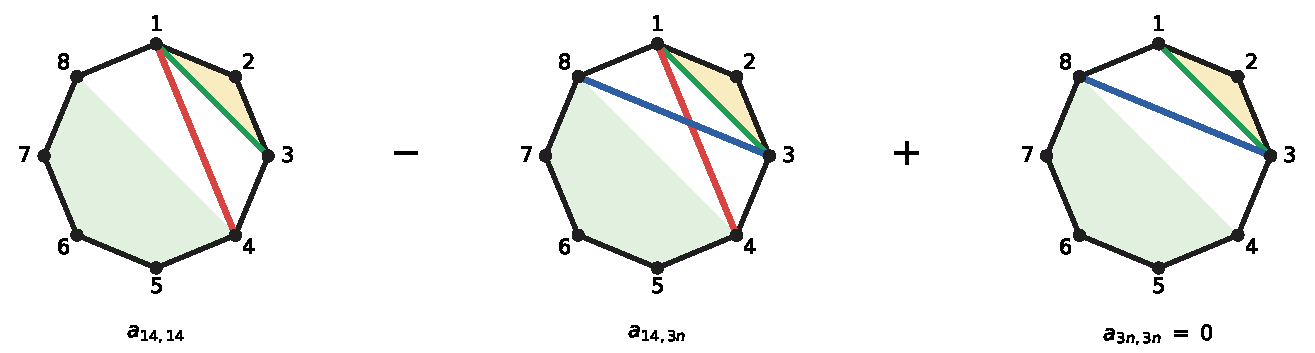
\includegraphics[width=0.95\textwidth]{figures/binomial_trace.pdf}
  \caption{The order--$2$ binomial trace at $k=2$, $n=8$: the three diagrams with two special/bare
  factors sum to zero. The same identity holds inside every D--subset (multiply each diagram by a
  common born--free factor).}
  \label{fig:bintrace}
\end{figure}

\noindent For $m=1$ the binomial trace is the \textbf{unitarity relation}
\begin{equation}\label{eq:unit}
  a_s\;-\;a_b\;=\;0,\qquad\text{i.e.}\quad a_{\X{1,k+2}}=a_{\X{k+1,n}}.
\end{equation}
At $k=1$ this is the familiar $a_{13}=a_{2n}$ of Part~I; at $k=2$ it is $a_{14}=a_{3n}$; at $k=3$,
$a_{15}=a_{4n}$. For $m=2$ it is the new quadratic relation $a_{ss}-a_{sb}+a_{bb}=0$, which at
$k=2$ reads $a_{14,14}-a_{14,3n}+a_{3n,3n}=0$ (Figure~\ref{fig:bintrace}); at $k=3$,
$a_{15,15}-a_{15,4n}+a_{4n,4n}=0$. For $m=3$ it is the cubic $a_{sss}-a_{ssb}+a_{sbb}-a_{bbb}=0$.

\section{The $1$--zero, recovered}
For $k=1$ the only offset is the special itself; the boundary propagators are
$\{\X{13},\X{1\ell},\X{2\ell},\X{2n}\}$ with $\ell=4,\dots,n-1$. The Step--$2$ relations are:
\begin{description}[topsep=2pt,itemsep=2pt,leftmargin=2em]
  \item[$m=1$ (1 BP).] Substituting $\X{2\ell}=\X{1\ell}-s$ and $\X{2n}=-s$ into the 1 BP piece
  $B_n^{(1)}\!=\!\frac{a_{13}}{\X{13}}+\sum_\ell\frac{a_{1\ell}}{\X{1\ell}}+\sum_\ell\frac{a_{2\ell}}{\X{2\ell}}+\frac{a_{2n}}{\X{2n}}$
  and collecting the $1/s$ piece gives $a_{13}-a_{2n}=0$, the binomial trace at $m=1$. The
  remaining $\sum_\ell a_{1\ell}/\X{1\ell}+\sum_\ell a_{2\ell}/\X{2\ell}=0$ is a polynomial in the
  independent variables $\X{1\ell}$ (after substituting $\X{2\ell}=\X{1\ell}-s$ at $s\to0$), forcing
  $a_{1\ell}=a_{2\ell}=0$ for all $\ell$ -- the Step--$1$ locality kill of Part~I, recovered.
  \item[$m=2$ (2 BP).] The leading $1/s^2$ piece gives the binomial trace $a_{13,13}-a_{13,2n}+a_{2n,2n}=0$.
  The next order in $s$ produces the per--column relations
  $a_{13,1\ell}-a_{2n,1\ell}-a_{1\ell,2\ell}=0$ (from the $\X{1\ell}\to0$ cut) and
  $a_{13,2\ell}-a_{2n,2\ell}+a_{1\ell,2\ell}=0$ (from $\X{2\ell}\to0$), which together force
  $a_{13,1\ell}+a_{13,2\ell}=a_{2n,1\ell}+a_{2n,2\ell}$ and produce the D--subset unitarity
  relations among the local triangulation coefficients (Part~I, $\S2$ of note~18).
\end{description}
The $1$--zero Step--$2$ system at $m=3$ proceeds analogously and is recorded in note~26.

\section{The $2$--zero}
For $k=2$, set $s=\X{1,4}$ and $b=\X{3,n}$. The new ingredient is the offset $\X{2,4}$
(``column--$4$''), which couples the $\X{2\ell}$ to the $\X{1\ell}$ and to $\X{2n}$ via
$\X{2\ell}=\X{1\ell}-s+\X{2,4}$ and $\X{2n}=-s+\X{2,4}$.

\paragraph{$m=1$ (1 BP).}
The boundary--propagator piece is
\begin{equation*}
  B_n^{(1)}\big|_{\Z^{(2)}}
  =\frac{a_{14}-a_{3n}}{s}+\sum_{\ell=5}^{n-1}\Big(\frac{a_{1\ell}}{\X{1\ell}}+\frac{a_{3\ell}}{\X{3\ell}}\Big)+\sum_{\ell=4}^{n}\frac{a_{2\ell}}{\X{2\ell}}\;=\;0.
\end{equation*}
Multiplying by $s$ and letting $s\to0$ extracts the binomial trace
\begin{equation}\label{eq:2zerounit}
  a_{14}=a_{3n}.
\end{equation}
The remainder is then a polynomial in $\X{1\ell},\X{2\ell},\X{3\ell},\X{2,4},\X{2n}$ that vanishes
identically, forcing $a_{1\ell}=a_{3\ell}=a_{2\ell}=0$ for all relevant $\ell$. \\
\emph{Step--$1$ recovered:} the kill at the $2$--zero, in Part~II's language regime~$A$ or~$B$,
follows automatically from this BP--graded D--subset decomposition.

\paragraph{$m=2$ (2 BP).}
The leading $1/s^2$ piece gives the new quadratic
\begin{equation}\label{eq:2zeroquad}
  \boxed{\;a_{14,14}+a_{3n,3n}-a_{14,3n}\;=\;0.\;}
\end{equation}
At the next order, after substituting $b=-s$ and $\X{i\ell}=\X{1\ell}-s+\X{i,k+2}$ etc.\ and
collecting the $1/s$ piece, three independent linear combinations appear; the $\X{2,4}\to0$ cut
(which forces $\X{2\ell}=\X{1\ell}$ and $\X{2n}=-s$) extracts the per--column relation
\begin{equation}\label{eq:2zerocol}
  a_{14,1\ell}+a_{14,2\ell}+a_{14,3\ell}\;-\;a_{3n,1\ell}-a_{3n,2\ell}-a_{3n,3\ell}\;=\;0,
  \qquad \ell=5,\dots,n-1;
\end{equation}
and the $\X{2,4}=\X{2n}$ cut (which holds when $s=0$) extracts the \emph{offset relation}
\begin{equation}\label{eq:2zerooffset}
  a_{14,24}+a_{14,2n}\;-\;a_{3n,24}-a_{3n,2n}\;=\;0.
\end{equation}
Together with \eqref{eq:2zeroquad}, equations \eqref{eq:2zerocol}--\eqref{eq:2zerooffset} exhaust
the $2$ BP D--subset (modulo born--free choices, which apply uniformly).

\begin{figure}[t]
  \centering
  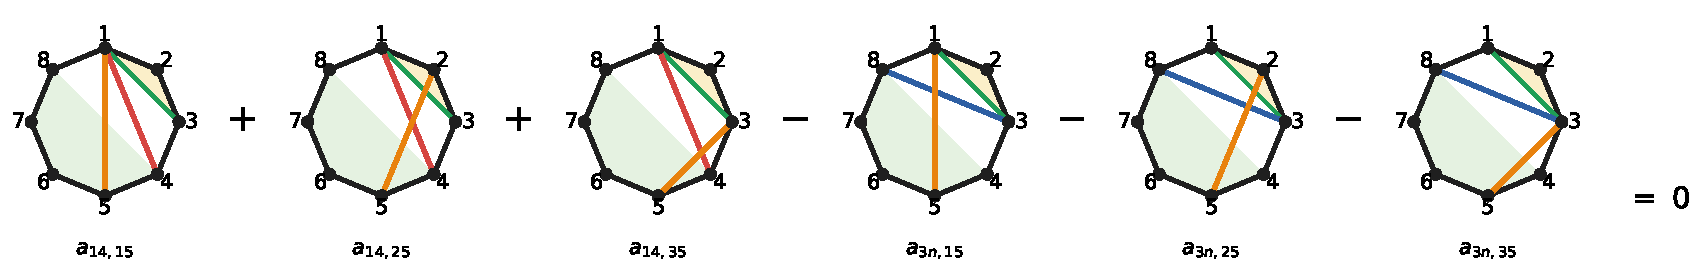
\includegraphics[width=0.96\textwidth]{figures/column_relation.pdf}
  \caption{The $2$--zero $2$ BP per--column relation \eqref{eq:2zerocol}, here $\ell=5$, drawn as
  six diagrams. The three terms paired with the special $\X{1,4}$ (left) cancel against the three
  paired with the bare $\X{3,n}$ (right). One such identity holds per $\ell\in\{5,\dots,n{-}1\}$,
  and inside every D--subset.}
  \label{fig:column}
\end{figure}

\paragraph{$m=3$ (3 BP).}
The leading $1/s^{3}$ piece gives the cubic binomial trace
\begin{equation}\label{eq:2zerocubic}
  a_{14,14,14}-a_{14,14,3n}+a_{14,3n,3n}-a_{3n,3n,3n}=0.
\end{equation}
The next power in $s$ produces the offset cubic
\begin{equation}\label{eq:2zerooffsetcubic}
  a_{14,14,24}+a_{14,14,2n}-a_{14,3n,24}-a_{14,3n,2n}+a_{3n,3n,24}+a_{3n,3n,2n}\;=\;0,
\end{equation}
and the per--column cubic
\begin{equation}\label{eq:2zerocolcubic}
  \sum_{i=1}^{3}\big(\,a_{14,14,i\ell}\;-\;a_{14,3n,i\ell}\;+\;a_{3n,3n,i\ell}\,\big)\;=\;0,
  \qquad \ell=5,\dots,n-1.
\end{equation}
The pattern continues: at every $m$ the leading $1/s^m$ piece is the binomial trace, and the
subleading pieces produce per--column and per--offset relations indexed by which $X\!\to\!0$ cut is
taken.

\section{The $3$--zero}
For $k=3$, set $s=\X{1,5}$, $b=\X{4,n}$, and two offsets $\X{2,5}, \X{3,5}$. By the same procedure:
\paragraph{$m=1$.} $a_{15}=a_{4n}$, plus $a_{i\ell}=0$ for all other 1 BP coefficients.
\paragraph{$m=2$.} The binomial trace $a_{15,15}-a_{15,4n}+a_{4n,4n}=0$, the per--column relation
$\sum_{i=1}^{4}\big(a_{15,i\ell}-a_{4n,i\ell}\big)=0$ for each $\ell=6,\dots,n-1$, and the
\emph{offset pair} relations
\begin{equation}\label{eq:3zerooffset}
  a_{15,i5}+a_{15,in}-a_{4n,i5}-a_{4n,in}\;=\;0,\qquad i=2,3,
\end{equation}
obtained from the $\X{i5}\to0$ cut (which sends $\X{i5}\!\to\!0$ and $\X{in}\!\to\!0$ after also
$\X{15}\!=\!0$).
\paragraph{Higher $m$.} The same pattern: the leading order yields the binomial trace, the next
orders yield per--column and per--offset relations. The number of relations grows linearly with $n$
(one per column $\ell$) and is fixed in $k$ (one binomial trace, $k-1$ offset pairings).

\section{The general pattern}
\begin{theorem}[Structure at order $m$]\label{thm:struct}
For each $k$, $n$, and $m\ge1$, the $k$--zero Step--$2$ relations at $|M|_{\mathrm{BP}}=m$ are
\begin{enumerate}[label=\textnormal{(\arabic*)},topsep=2pt,itemsep=1pt]
  \item \emph{the binomial trace} \eqref{eq:bintrace} (one relation);
  \item \emph{the per--column relations} of the form
  $\sum_{i\in\text{column }\ell}(\pm)\,a_{\square,\dots,\square,\,i\ell}=0$,
  one for each $\ell\in\{k{+}3,\dots,n{-}1\}$, with the $\square$ slots filled by some choice of
  $m-1$ further boundary--propagator factors;
  \item \emph{the offset relations}, one for each offset $\X{i,k+2}$ ($i=2,\dots,k$), pairing
  it with $\X{in}$ through the rate identification $\X{in}=\X{i,k+2}-s$;
\end{enumerate}
together with the lower--order relations carried by D--subsets that include further born--free
factors.
\end{theorem}
\begin{proof}[Proof sketch]
At fixed $m$ and D--subset, substituting \eqref{eq:constr} into $B_n^{(m)}|_{\Z^{(k)}}=0$ and
expanding in powers of $s$ yields a Laurent polynomial in the independent coordinates of
$\Z^{(k)}$. The coefficient of $1/s^m$ depends only on the $\{s,b\}$ pattern, giving
\eqref{eq:bintrace}. Coefficients of $1/s^{m-1}$ pick up linear factors from the offsets
$\X{i,k+2}$ and from the column variables $\X{1\ell}$. The $\X{1\ell}\!\to\!0$ cut isolates the
column--$\ell$ relation (which sums over $i=1,\dots,k{+}1$ since after $\X{1\ell}\!\to\!0$ the
constraints identify $\X{i\ell}=\X{i,k+2}$ uniformly). The $\X{i,k+2}\!\to\!0$ cut paired with
$\X{2n}\!\to\!0$ etc.\ isolates the offset relations.
\end{proof}

\section{Status: closing the system}
The combination of Part~II (all admissible asymptotic kills, indexed by the rate vector
$(\alpha_\ell;\beta_i)$) and the present Step--$2$ relations gives, for each pair $(k,n)$ and each
cyclic rotation, a closed linear system on the multiset coefficients $a_M$. Three structural facts
are immediate:
\begin{itemize}[topsep=2pt,itemsep=1pt]
  \item \textbf{Unitarity at every $k$.} The $m=1$ binomial trace \eqref{eq:unit} promotes the
  single $1$--zero unitarity $a_{13}=a_{2n}$ to a family $a_{\X{1,k+2}}=a_{\X{k+1,n}}$ valid for
  every $k$ and every cyclic rotation. Iterating across rotations identifies the coefficients of
  many triangulations.
  \item \textbf{Genuinely new relations at $k\ge2$.} The quadratic \eqref{eq:2zeroquad} and cubic
  \eqref{eq:2zerocubic} are not deducible from any cyclic rotation of the $1$--zero Step--$2$
  alone. They couple coefficients at one zone to coefficients at another (under cyclic rotation), and
  thereby refine the per--$n$ Laurent--cascade arguments of Part~I.
  \item \textbf{Polynomial growth of the system.} At fixed $m$ and $k$, the number of relations per
  zone grows as $O(n)$ (one per column plus $O(k)$ offsets); summed over $k=1,\dots,n-3$ and over
  $n$ cyclic rotations the total scales as $O(n^3)$. Whether the resulting system has trivial
  cokernel exactly on the triangulation coefficients is the all--$n$ locality conjecture.
\end{itemize}
The empirical data through $n=9$ (Part~I, $\S5$) and the explicit small--$n$ relations recorded in
notes~26--27 are consistent with this conjecture; a clean closed form for the kernel of the
combined Part~II + Part~III system is the next target.

\end{document}
